%\documentclass[10pt,handout]{beamer}
\documentclass[10pt]{beamer}
\usepackage[english]{babel} % Anpassa efter svenska. Ger svensk logga.
\usepackage[utf8]{inputenc} % Anpassa efter linux
\usepackage{graphicx}
\usetheme{Uppsala}
%\usecolortheme{UU} % Anpassa efter UU:s frger och logga
%\hypersetup{pdfpagemode=FullScreen} % Adobe Reader ska ppna fullskrm
\setbeamertemplate{itemize items}[circle]

% \usepackage{beamerthemesplit}
\usepackage{amsmath}
\usepackage{amssymb}
% \usepackage{graphics}
% \usepackage{graphicx}
% \usepackage{epsfig}
% \usepackage[latin1]{inputenc}
 \usepackage{color}
% \usepackage{fancybox}
% \usepackage{psfrag}
% \usepackage[english]{babel}
 \setbeamertemplate{footline}{\hfill\insertframenumber/\inserttotalframenumber}


%library(tinytex)
%tlmgr_install('csquotes')
\usepackage{csquotes}

%\usepackage{bm}
%\usepackage{natbib}
\newcommand{\bfm}[1]   {\mbox{\boldmath{${#1}$}}}
\newcommand{\Prob}   {\mbox{\textnormal{P}}}
\def\eqd{\,{\buildrel d \over =}\,}
\DeclareMathOperator{\E}{\mathbb{E}}

%%%%%%%%%%%%%%%%%%%%%%%%%%%%%%%%%%%%%%%%%%%%%%%%%%%%%%%%%%%%%%%%%%

\setlength{\parskip}{3mm}
\title[]{{\color{black}Machine learning, big data and artificial intelligence -- Block 4}}
\author[]{M{\aa}ns Magnusson\\Department of Statistics, Uppsala University}
\date{November 2020}


\begin{document}

\frame{\titlepage
% \thispagestyle{empty}
}



%%%%%%%%%%%%%%%%%%%%%%%%%%%%%%%%%%%%%%%%%%%%%%%%%%%%%%%%%%%%%%%%%%



\begin{frame}{Evaluation assignment 2}
\begin{itemize}
\item Took too much time (roughly 26h) - how to solve this? Hints? remove subtasks?
\item More teaching on code
\item The bugs...
\item Minor comments:
\begin{itemize}
\item xgboost video
\item bigger diff between RF and bagging
\item more focus on the assignment on the lecture
\end{itemize}
\end{itemize}
\end{frame}

\begin{frame}{Grading of assignment 1}
\begin{itemize}
\item Why is SGD important?
\item Differece between unsupervised and supervised learning. Task or experience?
\end{itemize}
\end{frame}

\begin{frame}{Masters thesis proposals}
\begin{enumerate}
\item Evaluation of probabilistic programming frameworks
\item Predicting introductions in Swedish parliamentary protocols using BERT
\item Topic model inference: (Stochastic) variational inference and Gibbs sampling
\item Will Svenska akademins ordlista (SAOL) improve Swedish word embeddings?
\item Fine-tune a language model (BERT) on EDGAR-CORPUS
\item OCR-error detection using image and text classification
\end{enumerate}
\end{frame}

\section{Introduction to Neural Networks}

%%%%%%%%%%%%%%%%%%%%%%%%%%%%%%%%%%%%%%%%%%%%%%%%%%%%%%%%%%%%%%%%%%


\begin{frame}{This week's lecture}
\begin{itemize}
\item Feed-Forward Neural Networks
\end{itemize}
\end{frame}


\frame{\frametitle{The Hype: Computer Vision}

\begin{figure}[h]
\caption{ImageNet performance (Roessler, 2019)}
\centering
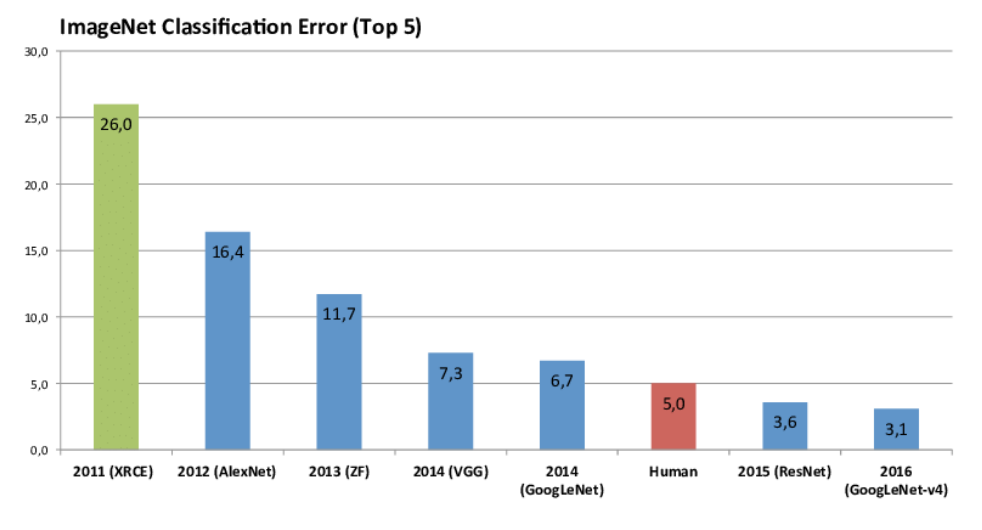
\includegraphics[width=0.8\textwidth]{fig/imageNet.png}
\end{figure}
}


\frame{\frametitle{The Hype: Speech Recognition}

\begin{figure}[h]
\centering
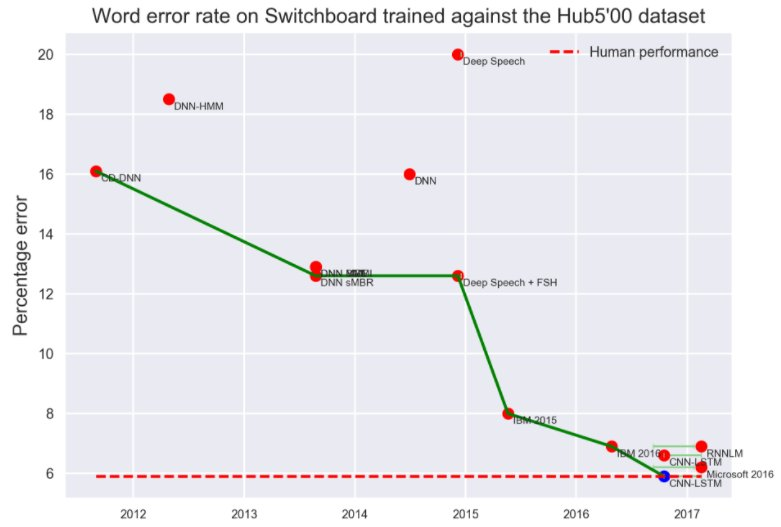
\includegraphics[width=0.8\textwidth]{fig/SP.jpeg}
\caption{Speech recognition performance (source: \url{https://eff.org/ai/metrics})}
\end{figure}
}

\frame{\frametitle{The Hype: Natural Language Processing}

\begin{figure}[h]
\centering
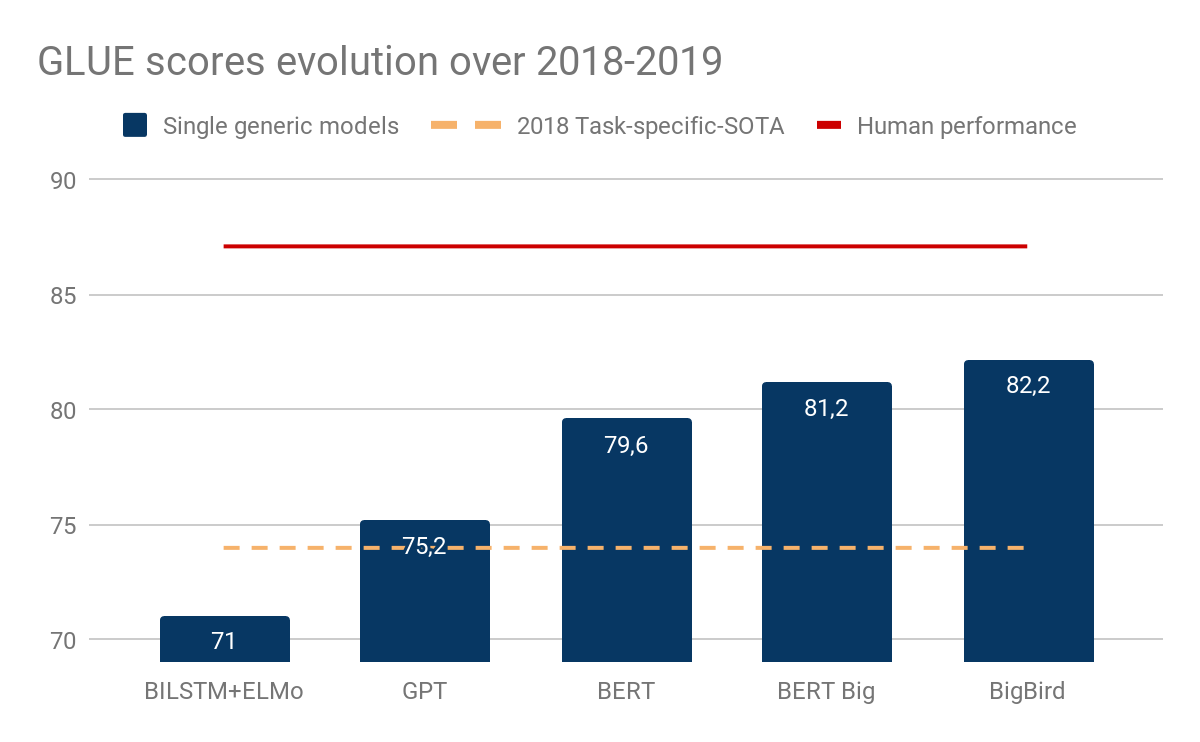
\includegraphics[width=0.8\textwidth]{fig/GLUE.png}
\caption{General Language Understanding (source: \url{https://www.programmersought.com/article/4251948498/})}
\end{figure}

Work is very much ongoing:

\url{https://gluebenchmark.com/leaderboard}


}

\frame{\frametitle{The Hype}

\begin{itemize}
\item Although - Neural Networks is not a silver bullet\pause
\item Remember the {\color{uured} Bayes error}\pause
\item Some times a linear regression (or Random Forest) is enough
\end{itemize}

}

\frame{\frametitle{The Feed-Forward Network}

\begin{figure}[h]
\centering
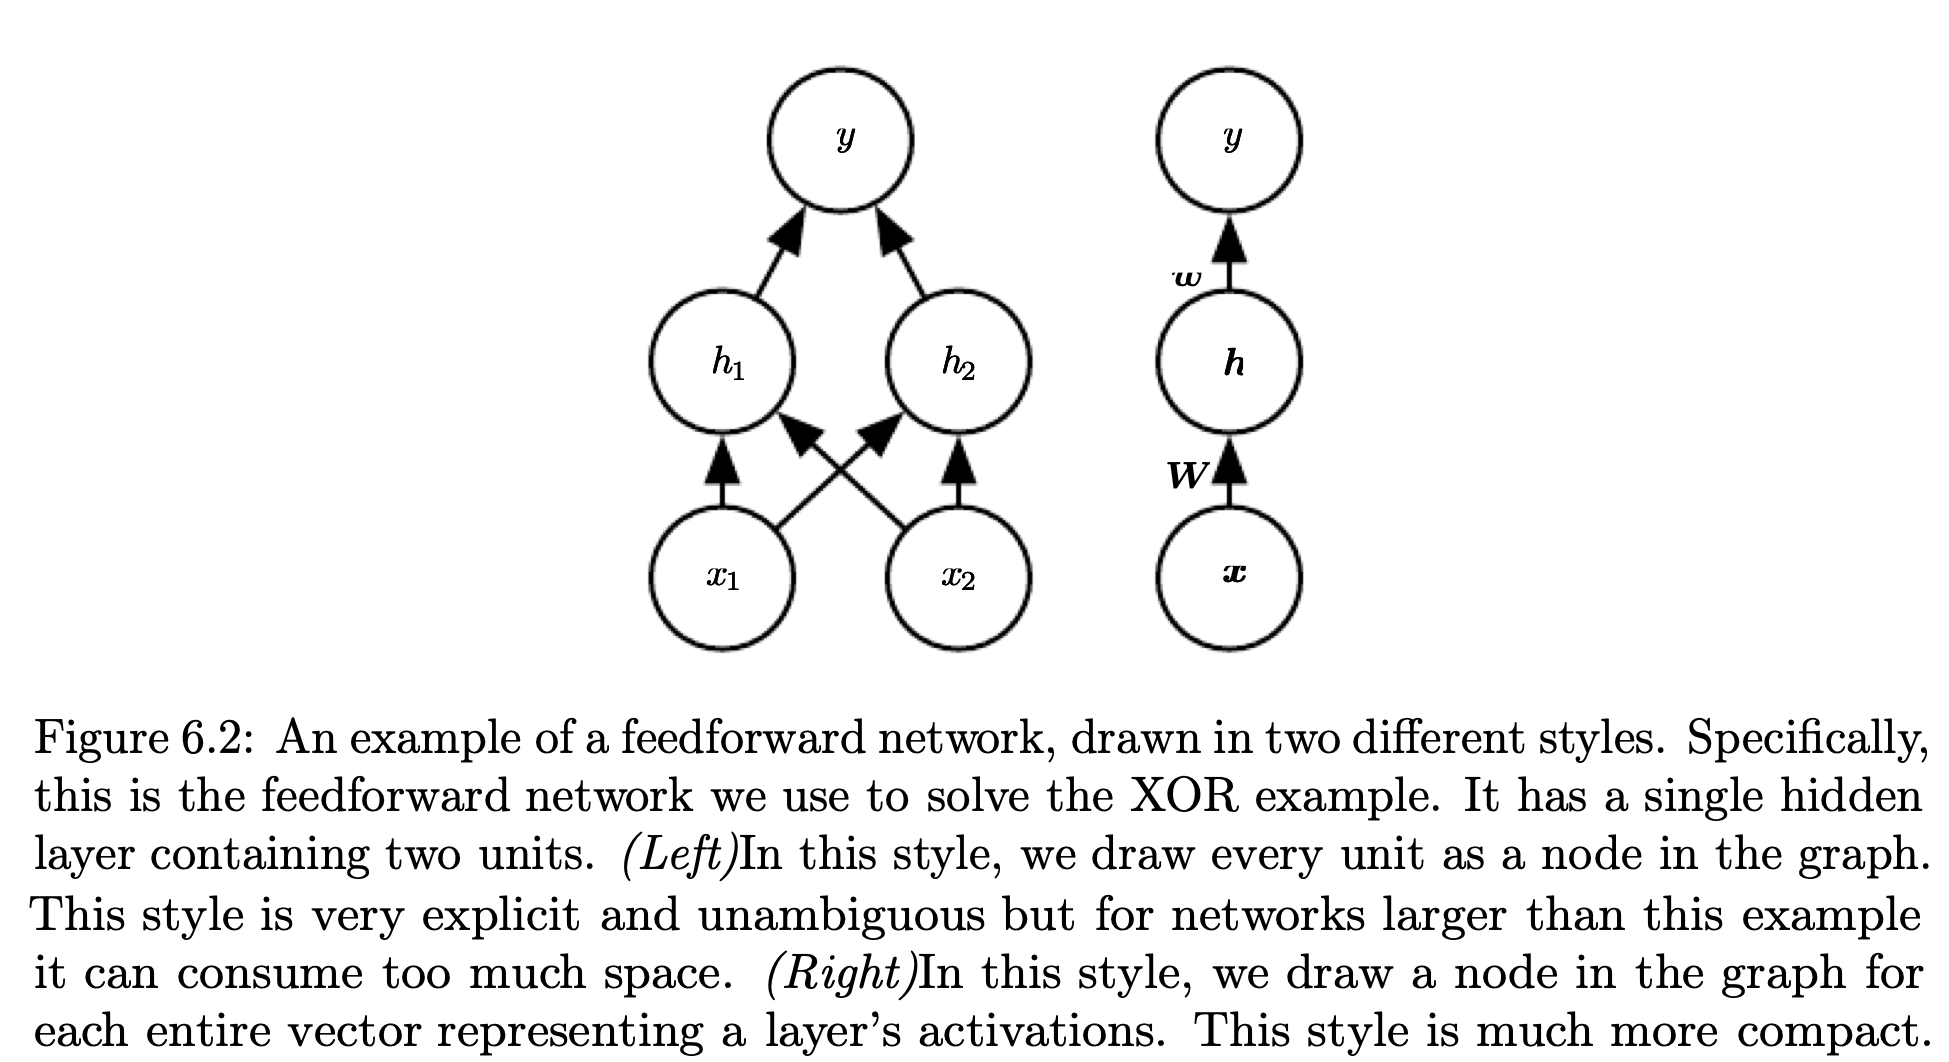
\includegraphics[width=0.8\textwidth]{fig/simple_NN.png}
\caption{A simple feed-forward network (Goodfellow et al, 2017)}
\end{figure}

{\color{uured} Important concepts}:

Layers, neurons, input, output, weights, bias, architecture

}

\frame{\frametitle{Different Architectures for Different Purposes}

\begin{itemize}
\item Different networks for different purposes
\begin{itemize}
\item {\color{uured} Convolutional Neural Networks}: Computer Vision\pause
\item {\color{uured} Recurrent Neural Networks}: Speech Audio (?)\pause
\item {\color{uured} Transformers/Attention}: Textual data
\end{itemize}
\item The Neural Network Zoo: \url{https://www.asimovinstitute.org/neural-network-zoo/}
\end{itemize}

}


\frame{\frametitle{Areas of Use: All fields}

\begin{itemize}
\item Supervised learning
\item Unsupervised learning
\item Reinforcement learning
\end{itemize}

}


\frame{\frametitle{Why and when neural nets?}

\begin{itemize}
\item Learning feature representations
\item Needs a lot of data to learn complex representations
\item Good for sensor data (high-dimensional)\pause
\item When should we not use neural networks?
\end{itemize}

}

\frame{\frametitle{Learning Representations}

\begin{figure}[h]
\centering
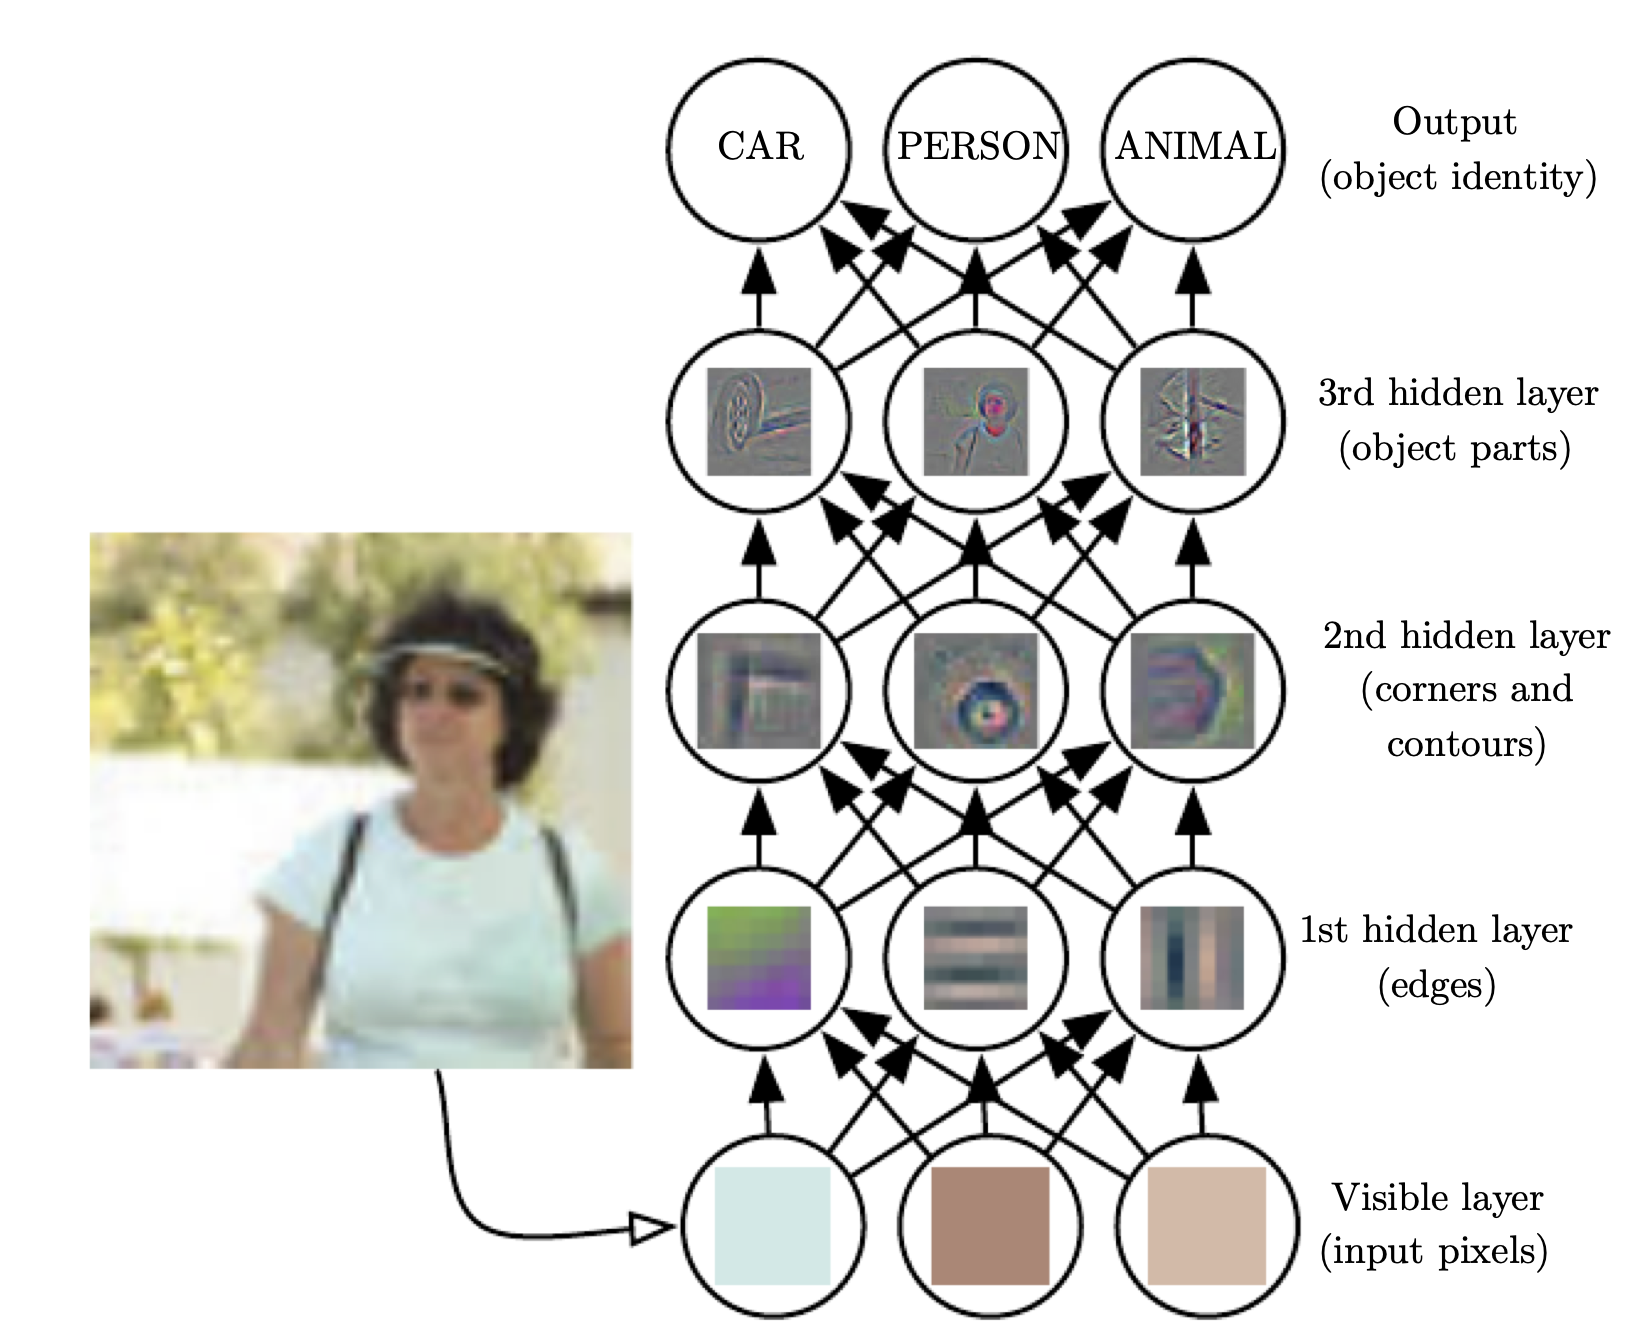
\includegraphics[width=0.8\textwidth]{fig/DL_fig_1_2_representations.png}
\caption{Learning representations can be crucial (Goodfellow et al, 2017, Fig. 1.2)}
\end{figure}

}




\subsection{Feed-Forward Neural Networks}
\frame{\frametitle{The Feed-Forward Network}

\begin{figure}[h]
\centering
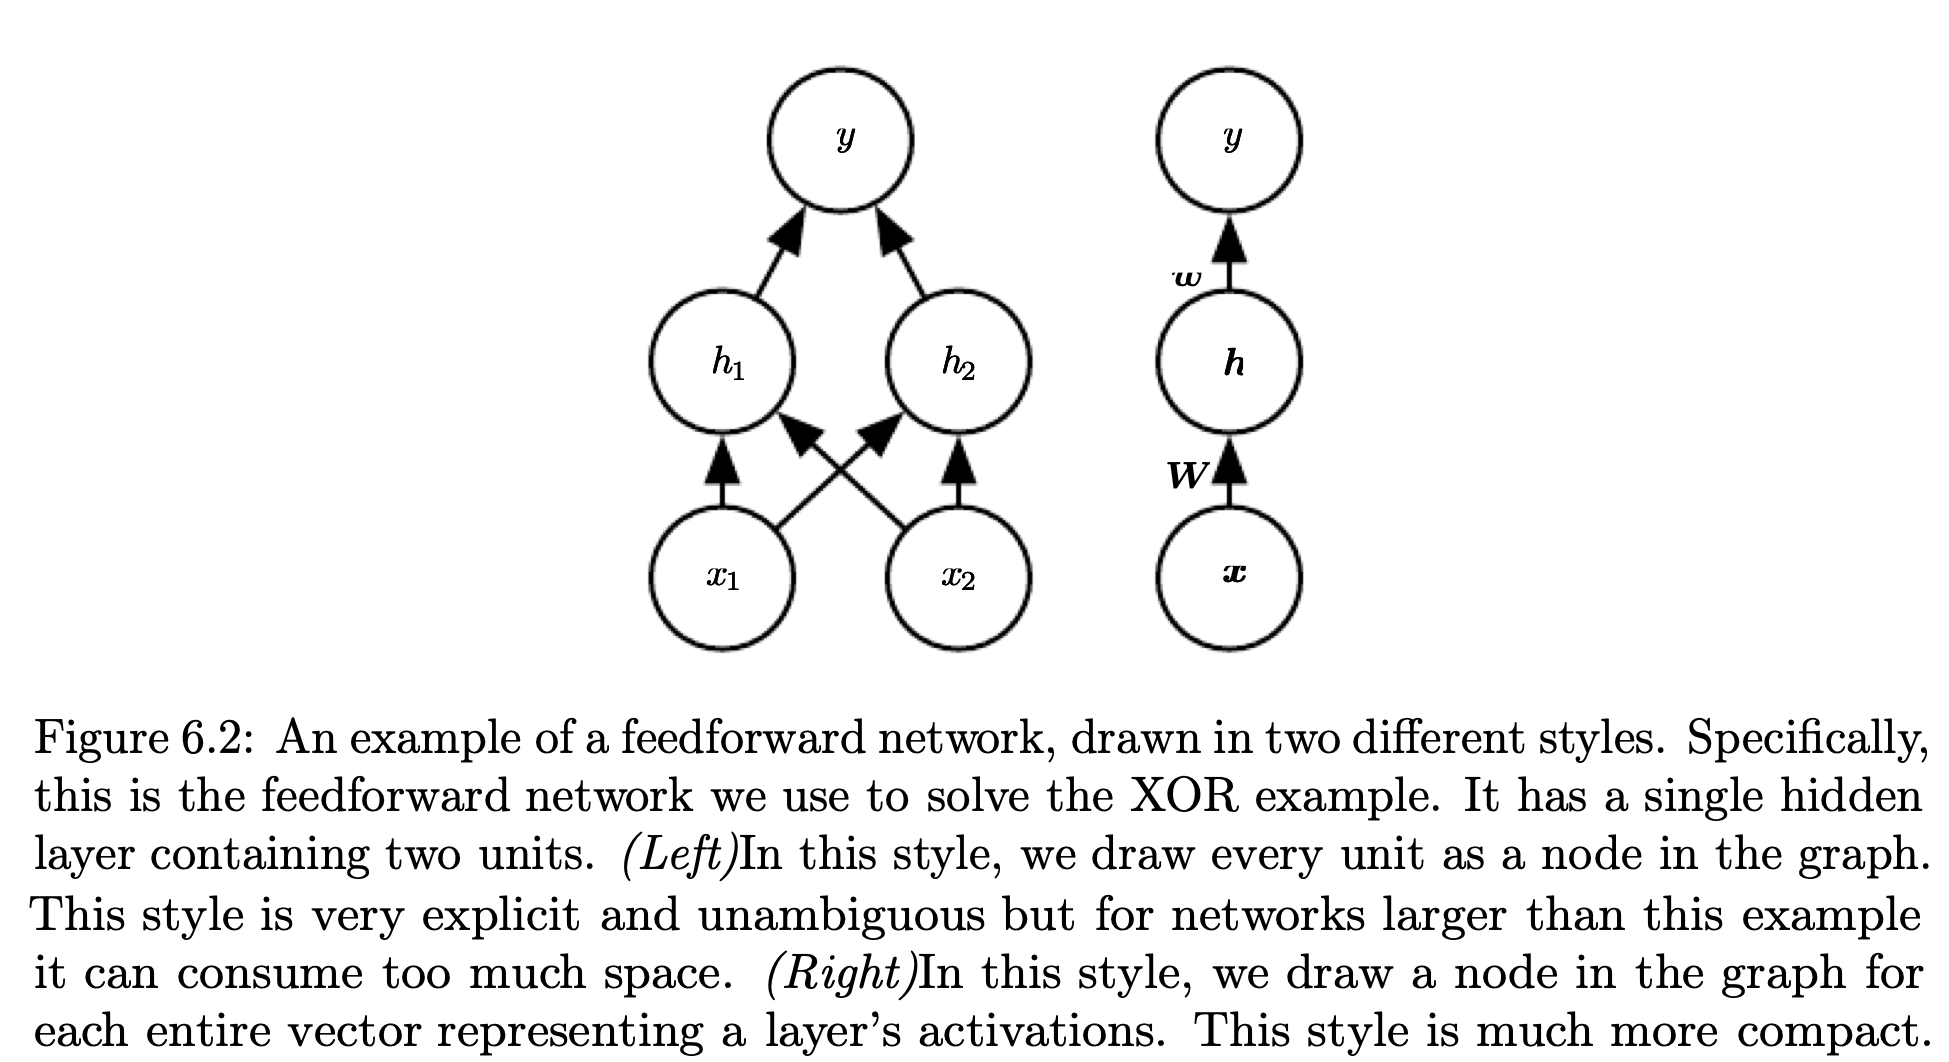
\includegraphics[width=0.8\textwidth]{fig/simple_NN.png}
\caption{A simple feed-forward network (Goodfellow et al, 2017, Fig. 6.2)}
\end{figure}

In mathematical notation:
\[
y_i = \mathbf{w}^T g(\mathbf{W}^T\mathbf{x}_i + \mathbf{b}_1) + \mathbf{b}_2
\]

}

\subsection{Feed-Forward Neural Networks}
\frame{\frametitle{The Feed-Forward Network}

\[
y_i = \mathbf{w}^T g(\mathbf{W}^T\mathbf{x}_i + \mathbf{b}_1) + \mathbf{b}_2
\]

\begin{equation*}
W =
\begin{pmatrix}
1 & 1 \\
1 & 1 \\
\end{pmatrix}
\,,w =
\begin{pmatrix}
1 \\
-2 \\
\end{pmatrix}\,,
b_1 =
\begin{pmatrix}
1 \\
-1 \\
\end{pmatrix}\,,
b_2 =
\begin{pmatrix}
0 \\
\end{pmatrix}
\end{equation*}

\begin{equation*}
g(z) = ReLU(z) = \max(0,z)\,,
x_i =
\begin{pmatrix}
0 \\
0 \\
\end{pmatrix}\,,
\end{equation*}

\[
y_i = \begin{pmatrix}
1 \\
-2 \\
\end{pmatrix}^T g(\begin{pmatrix}
0 \\
0 \\
\end{pmatrix} +
\begin{pmatrix}
1 \\
-1 \\
\end{pmatrix}
) + \begin{pmatrix}
0 \\
\end{pmatrix}
\]
\[
y_i = \begin{pmatrix}
1 \\
-2 \\
\end{pmatrix}^T \begin{pmatrix}
1 \\
0 \\
\end{pmatrix} + \begin{pmatrix}
0 \\
\end{pmatrix} = 1
\]

}



\frame{\frametitle{The Feed-Forward Network}

A feed-forward network for one observation ($x_i$).

\begin{align*}
\underbrace{\mathbf{h}_1}_{1 \times k_1} &= g_1(\underbrace{\mathbf{x}^{T}}_{1 \times p}\underbrace{\mathbf{W}_1}_{p \times k_1} + \underbrace{\mathbf{b}_1}_{1 \times k_1}) \\
& \vdots \\
\underbrace{\mathbf{h}_l}_{1 \times k_l}  &=  g_l(\underbrace{\mathbf{h}_{l-1}^{T}}_{1 \times k_{l-1}}\underbrace{\mathbf{W}_l}_{k_{l-1} \times k_l} + \underbrace{\mathbf{b}_l}_{1 \times k_l}) \\
& \vdots \\
\underbrace{\hat{\mathbf{y}}}_{1 \times m} &= g_{L}(\underbrace{\mathbf{h}^{T}_{{L-1}}}_{1 \times k_{l-1}}\underbrace{\mathbf{W}_{L}}_{k_{l-1} \times m} + \underbrace{\mathbf{b}_{L}}_{1 \times m})
\end{align*}

\[
\hat{y} = f_L(f_{L-1}(...f_1(x)...))
\]

% TODO Fix mathbf

}


\frame{\frametitle{Activation functions ($g_l$)}

\begin{itemize}
\item Sometimes use notation $\sigma$ as in $\sigma(W h + b)$\pause
\item Historically $g(z)$ has been the sigmoid or or hyperbolic tangent (tanh)\pause
\item Now, usually variants of Rectified linear unit (ReLU)
\begin{itemize}
\item $g(z)=\max{0,z}$
\item Easier to estimate with SGD
\item Easier for deep models
\end{itemize}
\item Last activation is the output function $g_L$, usually a softmax (if classification)
\[
f(z_i)={\frac {e^{z_i}}{\sum _{j=1}^{J}e^{z_{j}}}}
\]
\end{itemize}

}

\frame{\frametitle{Activation functions ($g_l$)}

\begin{figure}[h]
\centering
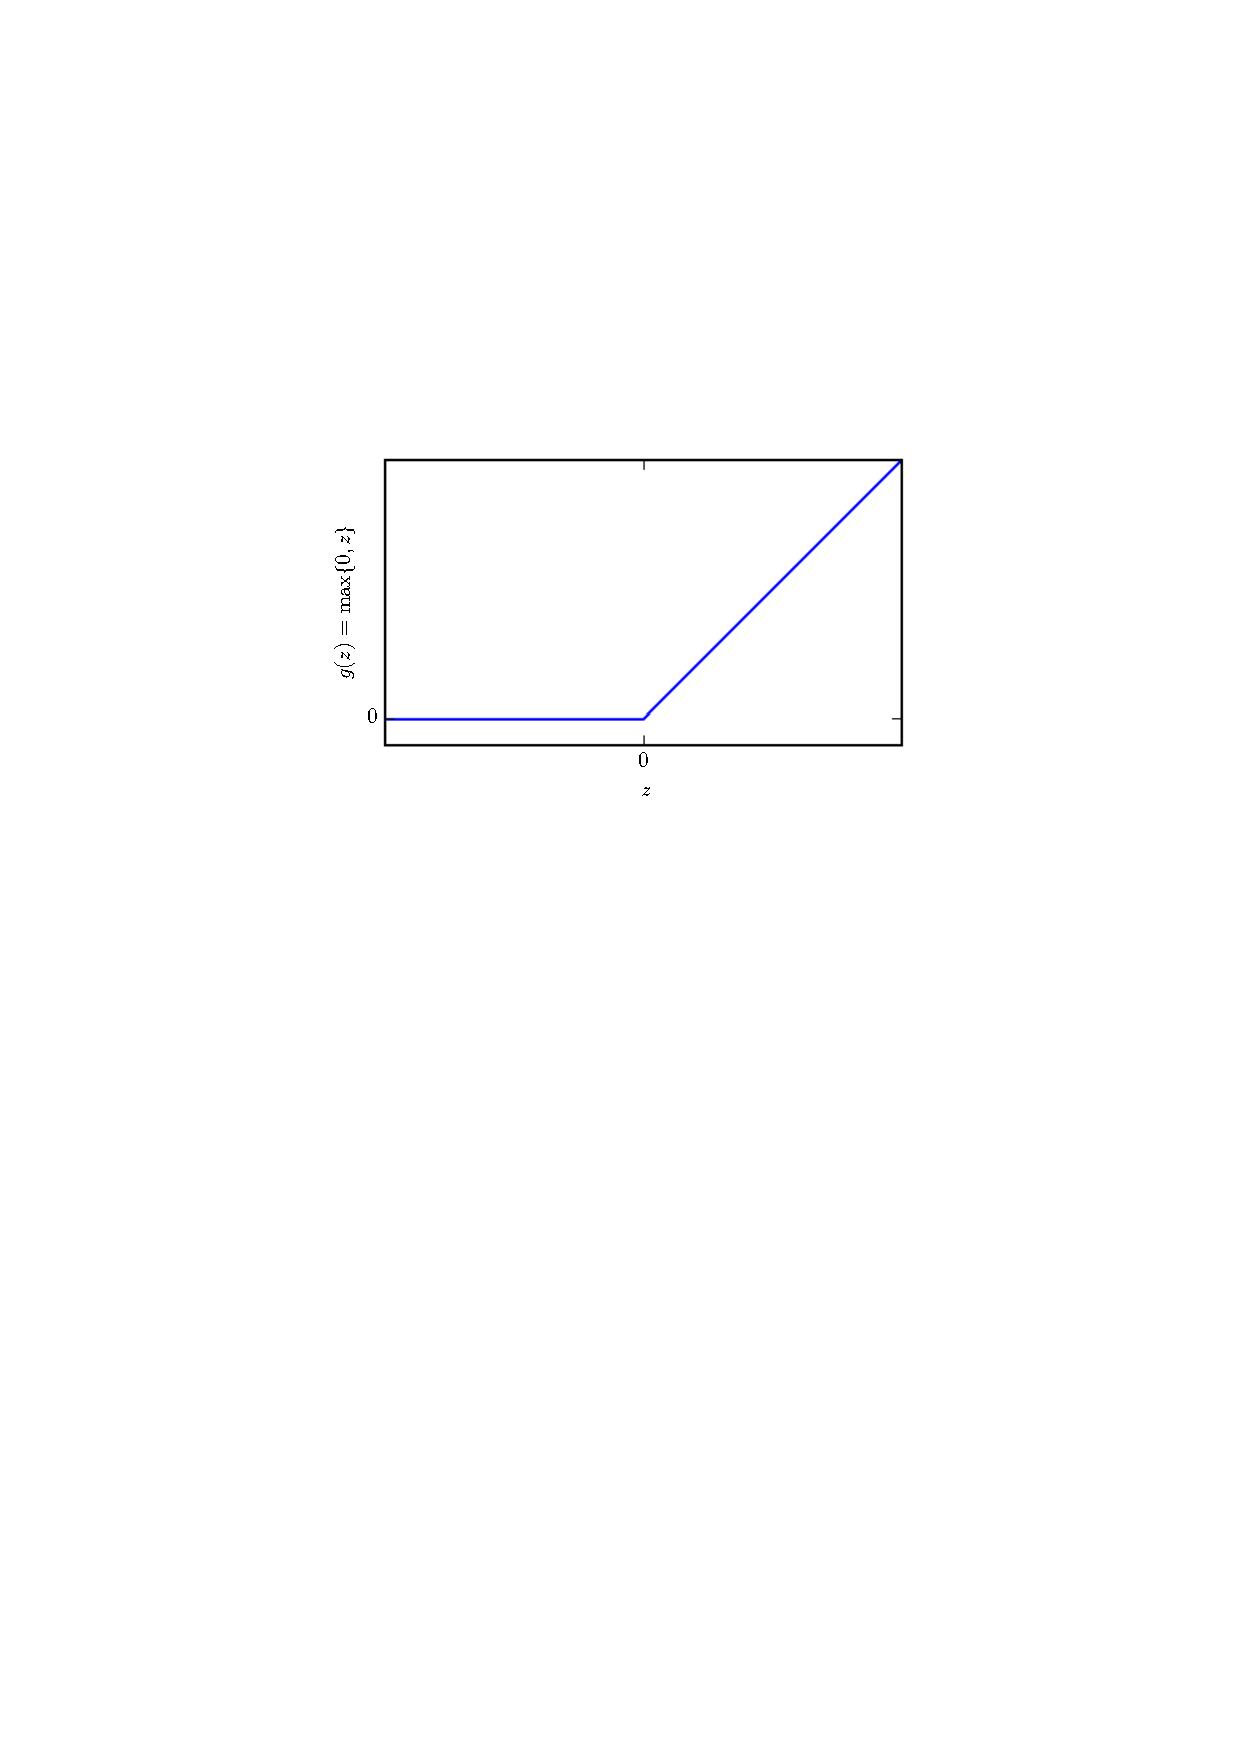
\includegraphics[width=0.6\textwidth]{fig/ReLu.pdf}
\caption{Rectified Linear Unit (Goodfellow et al, 2017, Fig. 6.3)}
\end{figure}

}


\frame{\frametitle{Universal Approximation Theorem}

"A feed-forward neural network with a linear output layer and at least one hidden layer with any 'squashing' activation function can approximate any Borel measurable function from one finite-dimensional space to another with any desired non-zero amount of error, provided that the network is given enough hidden units." (Goodfellow et al. 2017, p. 198)

\begin{itemize}
\item Also holds for ReLU
\item No garantuee we can learn the network
\item No garantuee that it will generalize
\item No indication of how large the network need to be
\end{itemize}

}

\subsection{Hyper-parameters}

\frame{\frametitle{Hyper-parameters in feed-forward networks}

\begin{itemize}
\item The number of layers
\item The number of neurons
\item Activation functions
\item The type of layers (CNN, MaxPooling, Multi-head attention)
\end{itemize}

}

\frame{\frametitle{How to choose parameters}

\begin{itemize}
\item Trial and error on validation sets
\item Art rather than science
\item Specialized approaches (Bayesian Optimization)\pause
\item Grid search (combinatorical explosion)
\begin{itemize}
\item Really bad with many parameters with less effects
\item If we have 5 irrelevant parameters we try 3 values for: 125 training per relevant run
\item Instead use...\pause
\end{itemize}
\item Random search
\end{itemize}

}

\frame{\frametitle{Grid search vs. Random Search}

\begin{figure}[h]
\centering
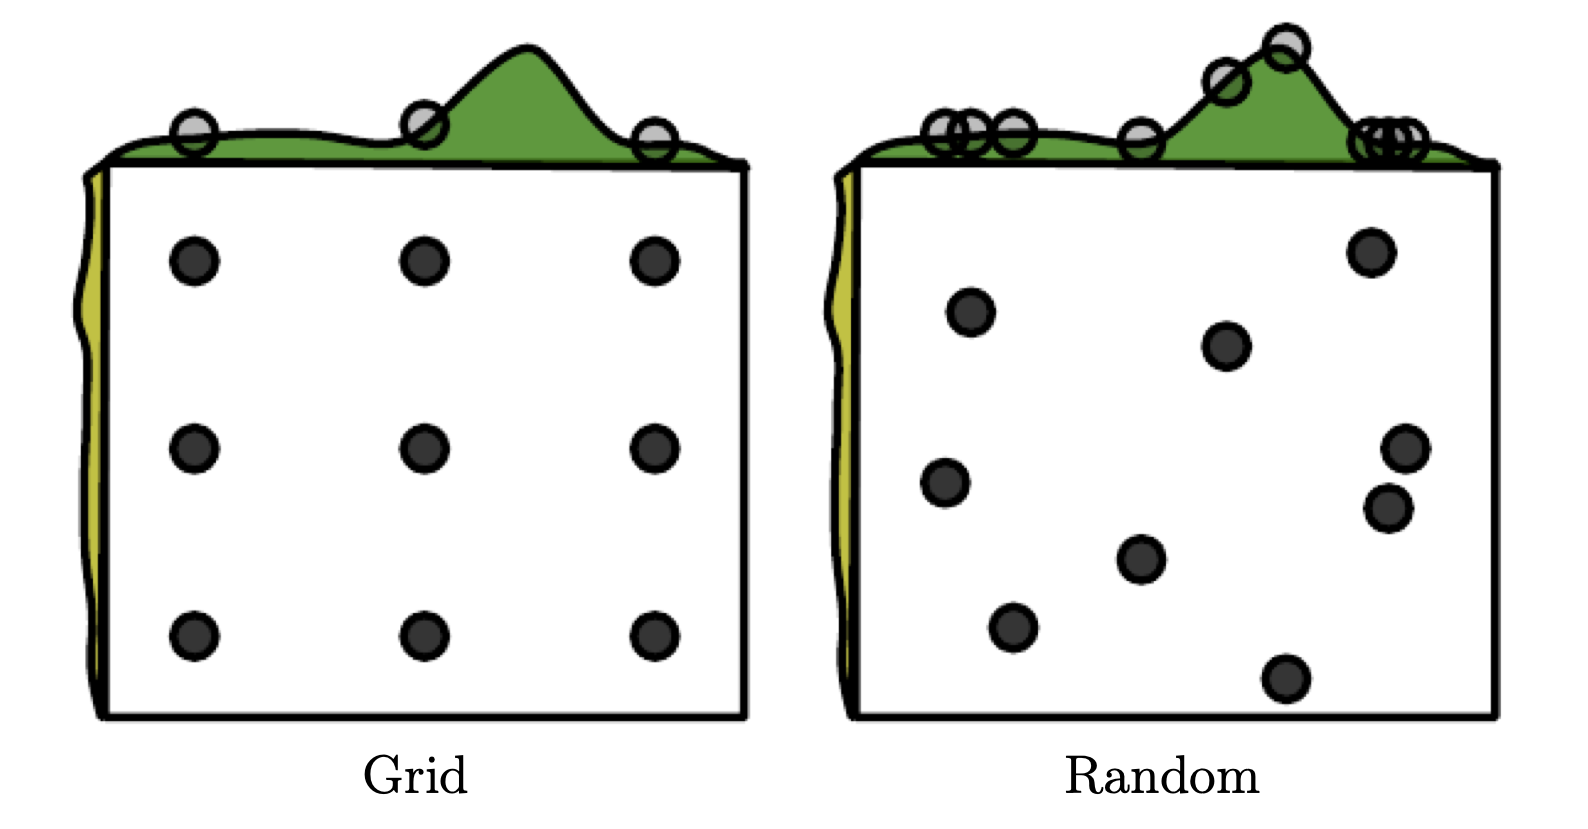
\includegraphics[width=0.6\textwidth]{fig/random_search.png}
\caption{Grid search and random search (Goodfellow et al, 2017, Fig. 11.2)}
\end{figure}

}


\section{Optimization}

\frame{\frametitle{Optimization of Neural Networks}

% TODO: Add the cost functions here (See DL and Keras)

\begin{itemize}
\item Difficult problem
\item Many local minima (weight space symmetry)
\item Platueas and sadel points
\begin{itemize}
\item Gradient is small - but not a minimum or maximum
\item Sadel points increases with the number of dimensions (?)
\item Large areas with small change in cost function
\end{itemize}
\end{itemize}

}

\frame{\frametitle{Optimization of Neural Networks II}

\begin{itemize}
\item A lot of parameters ($W$ and $b$)
\item Usually a lot of data\pause
\item Stochastic Gradient Descent, commonly
\begin{itemize}
\item Adam
\end{itemize}\pause
\item To compute gradients: backpropagation
\begin{itemize}
\item Chain-rule for derivatives
\end{itemize}

\end{itemize}

% TODO: Add slide on repetition on SGD here (take from block 1)

}

\frame{\frametitle{Initial values}

\begin{itemize}
\item We need to have starting values for SGD - non-trivial
\item Bad initial values might
\begin{itemize}
\item Bad convergence (local optimum)
\item Numerical problems
\end{itemize}
\item We want to break symmetry between layers
\item Initialization can be seen as a hyperparameter
\item Good practice
\begin{itemize}
\item Initialize values randomly close to zero (uniform or normal)
\end{itemize}
\end{itemize}

}


%\frame{\frametitle{Batch normalization}
%
%\begin{itemize}
%\item A way to simplify the optimization
%\end{itemize}
% TODO: Fix this part - add information here on batch normalization
%}



\frame{\frametitle{Neural Networks in Practice:\\ TensorFlow and Keras}
\begin{itemize}
\item Tensorflow
\begin{itemize}
\item Framework for large-scale machine learning and Neural Networks
\item Developed by Google
\item Computational graphs
\item Handles:
\begin{itemize}
\item Computing gradients for Neural Networks
\item Enable simple use of graphical processing units (GPU) and Tensor processing Units (TPU)
\item Used in both research and production
\end{itemize}
\end{itemize}
\item Keras
\begin{itemize}
\item Syntax for 'building' Neural Networks
\item Platform independent (ish)
\end{itemize}
\end{itemize}

\centering

\includegraphics[width=0.2\textwidth]{fig/TF_logo.png}

\includegraphics[width=0.2\textwidth]{fig/Keras_logo.png}

}

\section{Regularization}

\frame{\frametitle{Regularization of Neural Networks}

\begin{itemize}
\item Reduce traing error but improve test/validation error\pause
\item Neural Networks are extremely flexible / high model capacity\pause
\item Regularization is crucial for good generalizability of NN\pause
\end{itemize}

}

\frame{\frametitle{Weight decay / Norm penalty}

\begin{itemize}
\item Let
\[
\tilde{J}(W,b) = J(W,b) + \alpha \Omega(W)\,,
\]
where $J(W,b)$ is the cost function and $\alpha \Omega(W)$ is the penalty for the weight matrices.
\item $\alpha$ is the strength of the penalty.
\end{itemize}

}

\frame{\frametitle{Weight decay / Norm penalty}

\begin{itemize}
\item Let
\[
\Omega_1 (W) = \sum_i \sum_j |w|_{i,j}\,,
\]
and
\[
\Omega_2 (W) = \sum_i \sum_j w^2_{i,j}\,,
\]
be the $L_1$ and $L_2$ regularization respectively.
\item We can then get the cost function
\[
\tilde{J}(W,b) = J(W,b) + \sum_l \alpha_l \Omega_2(W_l)\,,
\]
\end{itemize}

}


\frame{\frametitle{Weight decay / Norm penalty}

\begin{itemize}
\item Lets define the cost function as
\begin{align*}
\tilde{J}(w) &= J(w) + \alpha \Omega_2(w)\\
             &= J(w) + \alpha w^T w
\end{align*}
\item Then the gradient update becomes
\begin{align*}
\nabla_w \tilde{J}(w) &= \nabla_w J(w) + 2\alpha w
\end{align*}
\item To update our weights with gradient descent
\begin{align*}
w \leftarrow & w - \epsilon( \nabla_w J(w) + 2\alpha w)\\
w \leftarrow & (1 - 2\alpha \epsilon)w - \epsilon \nabla_w J(w)\\
\end{align*}
\end{itemize}

}


\frame{\frametitle{Weight decay / Norm penalty}

\begin{figure}[h]
\centering
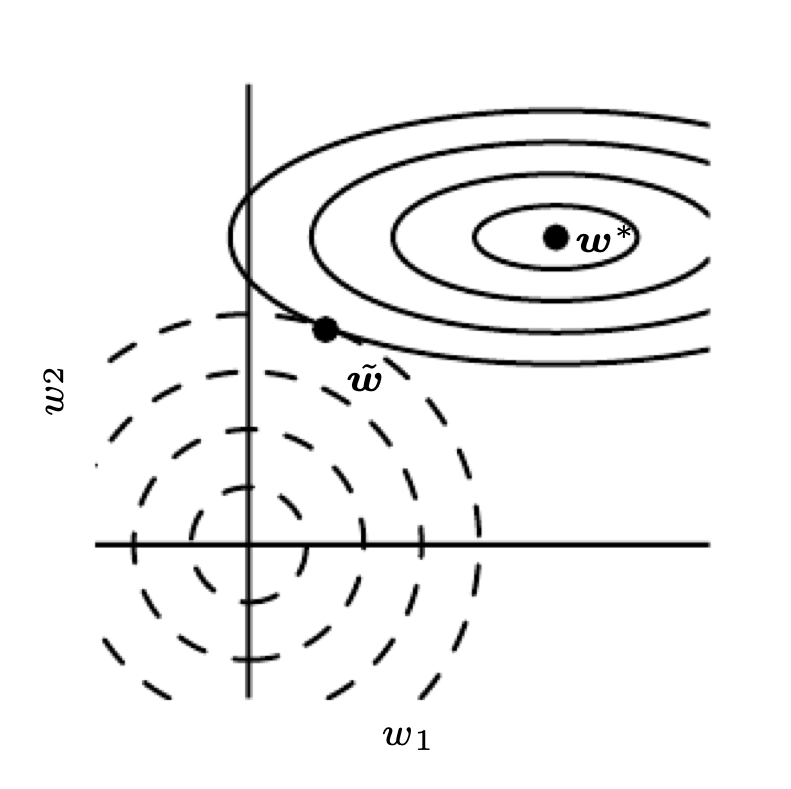
\includegraphics[width=0.6\textwidth]{fig/L2.png}
\caption{$L_2$ regularization (Goodfellow et al, 2017, Fig. 7.1)}
\end{figure}

}

\frame{\frametitle{Early Stopping}

\begin{itemize}
\item Stop optimization early based on validation error
\item Rerun to that number of epochs (hyperparameter)
\item Can be shown to be quivalent (under strict assumptions) to $L_2$ regularization
\end{itemize}

\begin{figure}[h]
\centering
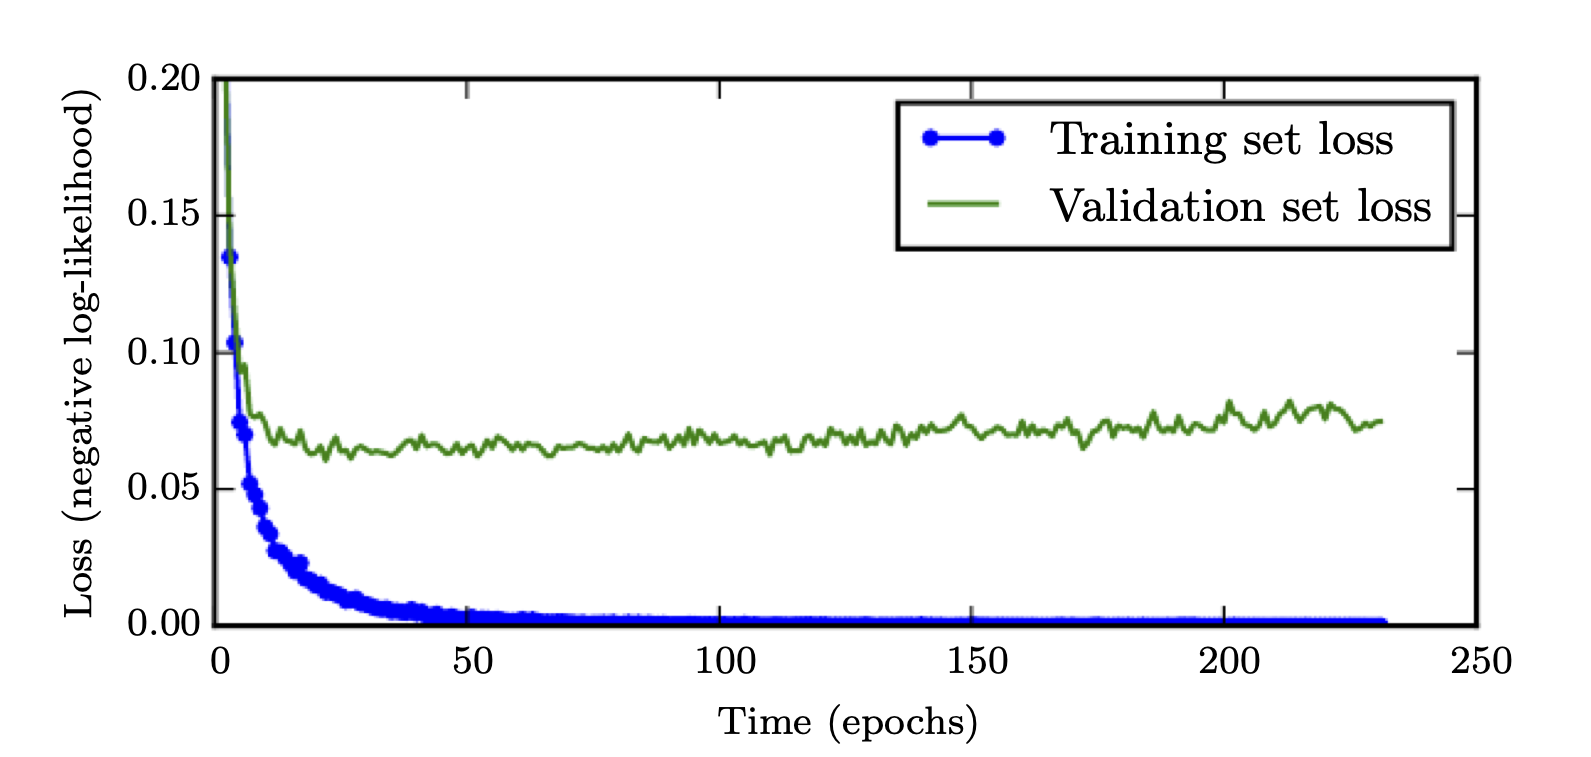
\includegraphics[width=0.8\textwidth]{fig/early_stopping.png}
\caption{Early Stopping (Goodfellow et al, 2017, Fig. 7.3)}
\end{figure}
}

\frame{\frametitle{Early Stopping}

\begin{figure}[h]
\centering
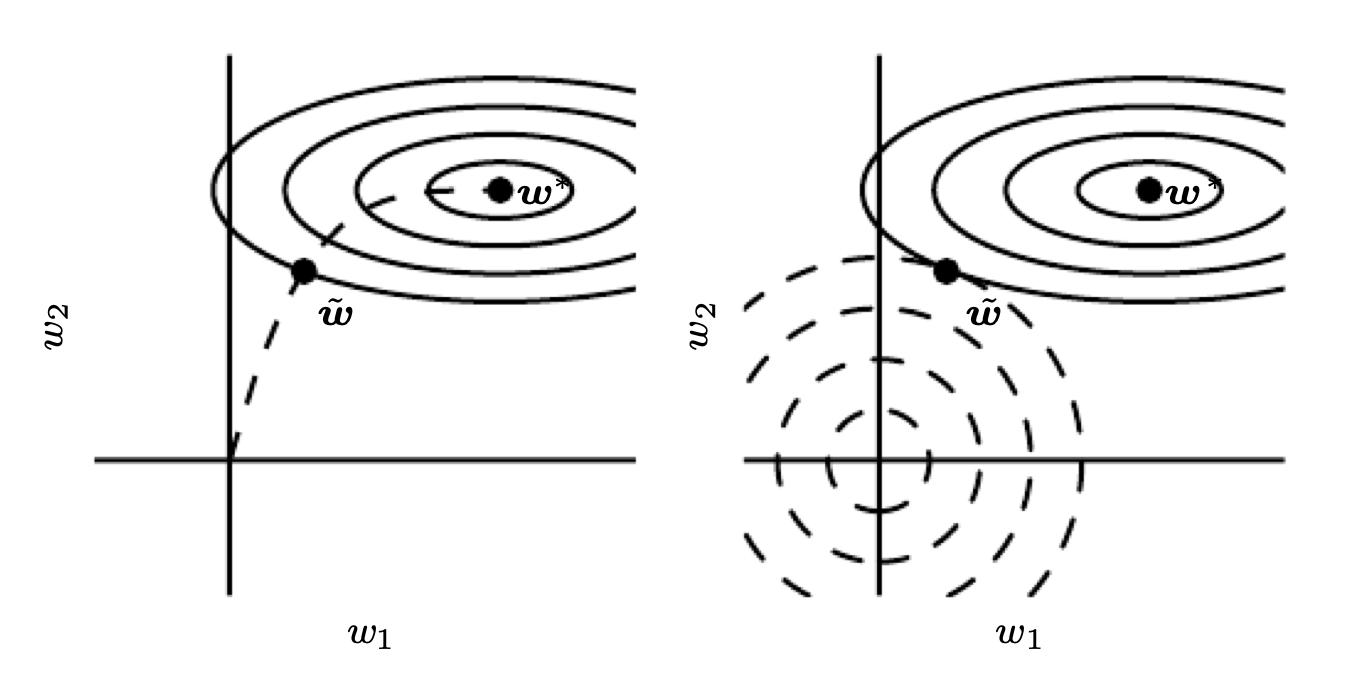
\includegraphics[width=0.8\textwidth]{fig/early_stopping_L2.png}
\caption{Early Stopping (Goodfellow et al, 2017, Fig. 7.4)}
\end{figure}
}

\frame{\frametitle{Dropout}

\begin{itemize}
\item In each iteration:
\begin{itemize}
\item Sample an indicator $I_i$ for each node $i$
\item Set the value $h_i$ to 0 with probability $p$
\end{itemize}
\item The dropout probability is typically 0.8 for input nodes and 0.5 for hidden nodes
\item Forces the network to
\begin{itemize}
\item not rely on individual nodes
\item spread out the weights over more nodes
\end{itemize}
\item Can be seen as an ensamble method
\end{itemize}
}


\frame{\frametitle{Dropout}


\begin{figure}[h]
\centering
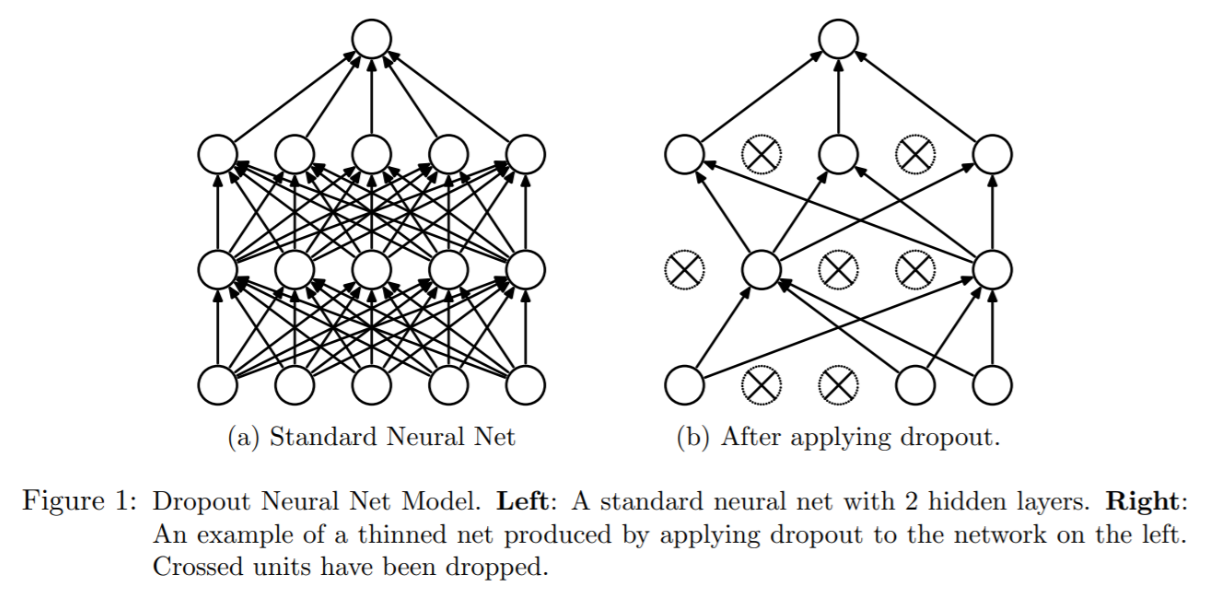
\includegraphics[width=1\textwidth]{fig/dropout.png}
\caption{Dropout (Srivastava et al, 2014)}
\end{figure}

}


\frame{\frametitle{Other regularization techniques}


\begin{itemize}
\item In CNN: Dataset augmentation
\item Get more data...
\end{itemize}

}

\end{document}
